% ═══════════════════════════════════════════════════════════════
% MIRAGE-UAS Paper Figures — Overleaf Setup Guide
%
% Required preamble (add to main.tex before \begin{document}):
% ═══════════════════════════════════════════════════════════════

\usepackage{tikz}
\usetikzlibrary{arrows.meta, positioning, shapes, calc, fit, backgrounds}

% Helper command used in attack model figure
\newcommand{\romark}[1]{\texttt{#1}}

% ═══════════════════════════════════════════════════════════════
% Usage in paper body:
%
%   % ═══════════════════════════════════════════════════════════════
% Figure: OpenClawAgent OODA Loop — Autonomous Deception Cycle
% Usage: % ═══════════════════════════════════════════════════════════════
% Figure: OpenClawAgent OODA Loop — Autonomous Deception Cycle
% Usage: % ═══════════════════════════════════════════════════════════════
% Figure: OpenClawAgent OODA Loop — Autonomous Deception Cycle
% Usage: \input{figures/fig_ooda_loop.tex}
% ═══════════════════════════════════════════════════════════════
\begin{figure}[t]
\centering
\resizebox{\columnwidth}{!}{%
\begin{tikzpicture}[
    >=stealth,
    node distance=2.8cm,
    phase/.style={
        rectangle, rounded corners=8pt, draw=black!80, line width=1.2pt,
        minimum width=3.2cm, minimum height=1.6cm, align=center,
        font=\sffamily\bfseries\small
    },
    observe/.style={phase, fill=blue!15, draw=blue!60},
    orient/.style={phase, fill=orange!15, draw=orange!60},
    decide/.style={phase, fill=green!15, draw=green!60},
    act/.style={phase, fill=red!15, draw=red!60},
    detail/.style={
        rectangle, rounded corners=4pt, draw=gray!50, fill=gray!5,
        font=\sffamily\scriptsize, align=left, text width=3.6cm,
        inner sep=4pt
    },
    autonomous/.style={
        rectangle, rounded corners=4pt, draw=purple!60, fill=purple!8,
        font=\sffamily\scriptsize, align=left, text width=3.2cm,
        inner sep=4pt, dashed
    },
    loopline/.style={->, line width=1.5pt, draw=black!70},
    detailline/.style={->, line width=0.6pt, draw=gray!60, dashed},
]

% ── OODA 4 phases (circular layout) ──────────────────────────
\node[observe] (O) at (0, 3.5) {OBSERVE\\[-2pt]{\footnotesize\textnormal{관찰}}};
\node[orient]  (R) at (5, 3.5) {ORIENT\\[-2pt]{\footnotesize\textnormal{판향}}};
\node[decide]  (D) at (5, 0)   {DECIDE\\[-2pt]{\footnotesize\textnormal{결정}}};
\node[act]     (A) at (0, 0)   {ACT\\[-2pt]{\footnotesize\textnormal{��동}}};

% ── Loop arrows ──────────────────────────────────────────────
\draw[loopline] (O) -- node[above, font=\sffamily\tiny, text=black!60] {fingerprint} (R);
\draw[loopline] (R) -- node[right, font=\sffamily\tiny, text=black!60] {phase+tool} (D);
\draw[loopline] (D) -- node[below, font=\sffamily\tiny, text=black!60] {strategy} (A);
\draw[loopline] (A) -- node[left, font=\sffamily\tiny, text=black!60] {feedback} (O);

% ── Center label ─────────────────────────────────────────────
\node[font=\sffamily\bfseries\footnotesize, text=purple!70] at (2.5, 1.75) {OpenClawAgent};
\node[font=\sffamily\tiny, text=gray!70] at (2.5, 1.35) {Autonomous OODA};

% ── Detail boxes ─────────────────────────────────────────────
% OBSERVE details
\node[detail] (Od) at (-3.8, 4.8) {
    \textbf{observe() / observe\_ws()}\\[2pt]
    \textbullet\ MAVLink msg\_type 추출\\
    \textbullet\ inter-arrival timing 측정\\
    \textbullet\ 명령 시퀀스 축적\\
    \textbullet\ 서비스 접촉 집합 갱신
};
\draw[detailline] (Od.east) -- (O.west);

% ORIENT details
\node[detail] (Rd) at (9.2, 4.8) {
    \textbf{\_detect\_tool() + \_detect\_phase()}\\[2pt]
    \textbullet\ nmap: interval$<$0.1s, cmds$>$5\\
    \textbullet\ mavproxy: HB$\times$2$\to$DATA\_STREAM\\
    \textbullet\ dronekit: SET\_MODE pattern\\
    \textbullet\ RECON$\to$EXPLOIT$\to$PERSIST$\to$EXFIL
};
\draw[detailline] (Rd.west) -- (R.east);

% DECIDE details
\node[detail] (Dd) at (9.2, -1.2) {
    \textbf{generate\_response()}\\[2pt]
    \textbullet\ RECON: rich telemetry\\
    \textbullet\ EXPLOIT: ACK(ACCEPTED)\\
    \textbullet\ PERSIST: operator STATUSTEXT\\
    \textbullet\ EXFIL: fake logs/config
};
\draw[detailline] (Dd.west) -- (D.east);

% ACT details
\node[detail] (Ad) at (-3.8, -1.2) {
    \textbf{MAVLink bytes / WS JSON}\\[2pt]
    \textbullet\ UDP sendto $\to$ 공격자\\
    \textbullet\ BeliefState 갱신\\
    \textbullet\ MTD urgency 평가\\
    \textbullet\ CTI event queue push
};
\draw[detailline] (Ad.east) -- (A.west);

% ── Autonomous behavior loops (bottom) ───────────────────────
\node[autonomous] (auto) at (2.5, -3.0) {
    \textbf{5 Autonomous Loops}\\[2pt]
    \textbullet\ proactive STATUSTEXT (15s)\\
    \textbullet\ sysid rotation (45s)\\
    \textbullet\ WS port rotation (90s)\\
    \textbullet\ mission refresh (60s)\\
    \textbullet\ param drift (45s)
};
\draw[detailline, draw=purple!50] (auto.north) -- (A.south);

% ── Confusion amplification ──────────────────────────────────
\node[autonomous] (conf) at (7.5, -3.0) {
    \textbf{Confusion Amplification}\\[2pt]
    \textbullet\ ghost port (services $\geq \theta$)\\
    \textbullet\ false flag (dwell $> \theta$)\\
    \textbullet\ ARM $\to$ takeoff $\to$ crash
};
\draw[detailline, draw=purple!50] (conf.north west) -- (D.south);

\end{tikzpicture}
}
\caption{OpenClawAgent OODA 자율 기만 루프. 4단계 관찰-판향-결정-행동 사이클이 공격자 도구(5종)와 공격 단계(4단계)를 실시간으로 식별하고 적응형 응답을 생성한다. 5개 독립 자율 행동 루프와 혼란 증폭 트리거가 병렬 실행된다.}
\label{fig:ooda}
\end{figure}

% ═══════════════════════════════════════════════════════════════
\begin{figure}[t]
\centering
\resizebox{\columnwidth}{!}{%
\begin{tikzpicture}[
    >=stealth,
    node distance=2.8cm,
    phase/.style={
        rectangle, rounded corners=8pt, draw=black!80, line width=1.2pt,
        minimum width=3.2cm, minimum height=1.6cm, align=center,
        font=\sffamily\bfseries\small
    },
    observe/.style={phase, fill=blue!15, draw=blue!60},
    orient/.style={phase, fill=orange!15, draw=orange!60},
    decide/.style={phase, fill=green!15, draw=green!60},
    act/.style={phase, fill=red!15, draw=red!60},
    detail/.style={
        rectangle, rounded corners=4pt, draw=gray!50, fill=gray!5,
        font=\sffamily\scriptsize, align=left, text width=3.6cm,
        inner sep=4pt
    },
    autonomous/.style={
        rectangle, rounded corners=4pt, draw=purple!60, fill=purple!8,
        font=\sffamily\scriptsize, align=left, text width=3.2cm,
        inner sep=4pt, dashed
    },
    loopline/.style={->, line width=1.5pt, draw=black!70},
    detailline/.style={->, line width=0.6pt, draw=gray!60, dashed},
]

% ── OODA 4 phases (circular layout) ──────────────────────────
\node[observe] (O) at (0, 3.5) {OBSERVE\\[-2pt]{\footnotesize\textnormal{관찰}}};
\node[orient]  (R) at (5, 3.5) {ORIENT\\[-2pt]{\footnotesize\textnormal{판향}}};
\node[decide]  (D) at (5, 0)   {DECIDE\\[-2pt]{\footnotesize\textnormal{결정}}};
\node[act]     (A) at (0, 0)   {ACT\\[-2pt]{\footnotesize\textnormal{��동}}};

% ── Loop arrows ──────────────────────────────────────────────
\draw[loopline] (O) -- node[above, font=\sffamily\tiny, text=black!60] {fingerprint} (R);
\draw[loopline] (R) -- node[right, font=\sffamily\tiny, text=black!60] {phase+tool} (D);
\draw[loopline] (D) -- node[below, font=\sffamily\tiny, text=black!60] {strategy} (A);
\draw[loopline] (A) -- node[left, font=\sffamily\tiny, text=black!60] {feedback} (O);

% ── Center label ─────────────────────────────────────────────
\node[font=\sffamily\bfseries\footnotesize, text=purple!70] at (2.5, 1.75) {OpenClawAgent};
\node[font=\sffamily\tiny, text=gray!70] at (2.5, 1.35) {Autonomous OODA};

% ── Detail boxes ─────────────────────────────────────────────
% OBSERVE details
\node[detail] (Od) at (-3.8, 4.8) {
    \textbf{observe() / observe\_ws()}\\[2pt]
    \textbullet\ MAVLink msg\_type 추출\\
    \textbullet\ inter-arrival timing 측정\\
    \textbullet\ 명령 시퀀스 축적\\
    \textbullet\ 서비스 접촉 집합 갱신
};
\draw[detailline] (Od.east) -- (O.west);

% ORIENT details
\node[detail] (Rd) at (9.2, 4.8) {
    \textbf{\_detect\_tool() + \_detect\_phase()}\\[2pt]
    \textbullet\ nmap: interval$<$0.1s, cmds$>$5\\
    \textbullet\ mavproxy: HB$\times$2$\to$DATA\_STREAM\\
    \textbullet\ dronekit: SET\_MODE pattern\\
    \textbullet\ RECON$\to$EXPLOIT$\to$PERSIST$\to$EXFIL
};
\draw[detailline] (Rd.west) -- (R.east);

% DECIDE details
\node[detail] (Dd) at (9.2, -1.2) {
    \textbf{generate\_response()}\\[2pt]
    \textbullet\ RECON: rich telemetry\\
    \textbullet\ EXPLOIT: ACK(ACCEPTED)\\
    \textbullet\ PERSIST: operator STATUSTEXT\\
    \textbullet\ EXFIL: fake logs/config
};
\draw[detailline] (Dd.west) -- (D.east);

% ACT details
\node[detail] (Ad) at (-3.8, -1.2) {
    \textbf{MAVLink bytes / WS JSON}\\[2pt]
    \textbullet\ UDP sendto $\to$ 공격자\\
    \textbullet\ BeliefState 갱신\\
    \textbullet\ MTD urgency 평가\\
    \textbullet\ CTI event queue push
};
\draw[detailline] (Ad.east) -- (A.west);

% ── Autonomous behavior loops (bottom) ───────────────────────
\node[autonomous] (auto) at (2.5, -3.0) {
    \textbf{5 Autonomous Loops}\\[2pt]
    \textbullet\ proactive STATUSTEXT (15s)\\
    \textbullet\ sysid rotation (45s)\\
    \textbullet\ WS port rotation (90s)\\
    \textbullet\ mission refresh (60s)\\
    \textbullet\ param drift (45s)
};
\draw[detailline, draw=purple!50] (auto.north) -- (A.south);

% ── Confusion amplification ──────────────────────────────────
\node[autonomous] (conf) at (7.5, -3.0) {
    \textbf{Confusion Amplification}\\[2pt]
    \textbullet\ ghost port (services $\geq \theta$)\\
    \textbullet\ false flag (dwell $> \theta$)\\
    \textbullet\ ARM $\to$ takeoff $\to$ crash
};
\draw[detailline, draw=purple!50] (conf.north west) -- (D.south);

\end{tikzpicture}
}
\caption{OpenClawAgent OODA 자율 기만 루프. 4단계 관찰-판향-결정-행동 사이클이 공격자 도구(5종)와 공격 단계(4단계)를 실시간으로 식별하고 적응형 응답을 생성한다. 5개 독립 자율 행동 루프와 혼란 증폭 트리거가 병렬 실행된다.}
\label{fig:ooda}
\end{figure}

% ═══════════════════════════════════════════════════════════════
\begin{figure}[t]
\centering
\resizebox{\columnwidth}{!}{%
\begin{tikzpicture}[
    >=stealth,
    node distance=2.8cm,
    phase/.style={
        rectangle, rounded corners=8pt, draw=black!80, line width=1.2pt,
        minimum width=3.2cm, minimum height=1.6cm, align=center,
        font=\sffamily\bfseries\small
    },
    observe/.style={phase, fill=blue!15, draw=blue!60},
    orient/.style={phase, fill=orange!15, draw=orange!60},
    decide/.style={phase, fill=green!15, draw=green!60},
    act/.style={phase, fill=red!15, draw=red!60},
    detail/.style={
        rectangle, rounded corners=4pt, draw=gray!50, fill=gray!5,
        font=\sffamily\scriptsize, align=left, text width=3.6cm,
        inner sep=4pt
    },
    autonomous/.style={
        rectangle, rounded corners=4pt, draw=purple!60, fill=purple!8,
        font=\sffamily\scriptsize, align=left, text width=3.2cm,
        inner sep=4pt, dashed
    },
    loopline/.style={->, line width=1.5pt, draw=black!70},
    detailline/.style={->, line width=0.6pt, draw=gray!60, dashed},
]

% ── OODA 4 phases (circular layout) ──────────────────────────
\node[observe] (O) at (0, 3.5) {OBSERVE\\[-2pt]{\footnotesize\textnormal{관찰}}};
\node[orient]  (R) at (5, 3.5) {ORIENT\\[-2pt]{\footnotesize\textnormal{판향}}};
\node[decide]  (D) at (5, 0)   {DECIDE\\[-2pt]{\footnotesize\textnormal{결정}}};
\node[act]     (A) at (0, 0)   {ACT\\[-2pt]{\footnotesize\textnormal{��동}}};

% ── Loop arrows ──────────────────────────────────────────────
\draw[loopline] (O) -- node[above, font=\sffamily\tiny, text=black!60] {fingerprint} (R);
\draw[loopline] (R) -- node[right, font=\sffamily\tiny, text=black!60] {phase+tool} (D);
\draw[loopline] (D) -- node[below, font=\sffamily\tiny, text=black!60] {strategy} (A);
\draw[loopline] (A) -- node[left, font=\sffamily\tiny, text=black!60] {feedback} (O);

% ── Center label ─────────────────────────────────────────────
\node[font=\sffamily\bfseries\footnotesize, text=purple!70] at (2.5, 1.75) {OpenClawAgent};
\node[font=\sffamily\tiny, text=gray!70] at (2.5, 1.35) {Autonomous OODA};

% ── Detail boxes ─────────────────────────────────────────────
% OBSERVE details
\node[detail] (Od) at (-3.8, 4.8) {
    \textbf{observe() / observe\_ws()}\\[2pt]
    \textbullet\ MAVLink msg\_type 추출\\
    \textbullet\ inter-arrival timing 측정\\
    \textbullet\ 명령 시퀀스 축적\\
    \textbullet\ 서비스 접촉 집합 갱신
};
\draw[detailline] (Od.east) -- (O.west);

% ORIENT details
\node[detail] (Rd) at (9.2, 4.8) {
    \textbf{\_detect\_tool() + \_detect\_phase()}\\[2pt]
    \textbullet\ nmap: interval$<$0.1s, cmds$>$5\\
    \textbullet\ mavproxy: HB$\times$2$\to$DATA\_STREAM\\
    \textbullet\ dronekit: SET\_MODE pattern\\
    \textbullet\ RECON$\to$EXPLOIT$\to$PERSIST$\to$EXFIL
};
\draw[detailline] (Rd.west) -- (R.east);

% DECIDE details
\node[detail] (Dd) at (9.2, -1.2) {
    \textbf{generate\_response()}\\[2pt]
    \textbullet\ RECON: rich telemetry\\
    \textbullet\ EXPLOIT: ACK(ACCEPTED)\\
    \textbullet\ PERSIST: operator STATUSTEXT\\
    \textbullet\ EXFIL: fake logs/config
};
\draw[detailline] (Dd.west) -- (D.east);

% ACT details
\node[detail] (Ad) at (-3.8, -1.2) {
    \textbf{MAVLink bytes / WS JSON}\\[2pt]
    \textbullet\ UDP sendto $\to$ 공격자\\
    \textbullet\ BeliefState 갱신\\
    \textbullet\ MTD urgency 평가\\
    \textbullet\ CTI event queue push
};
\draw[detailline] (Ad.east) -- (A.west);

% ── Autonomous behavior loops (bottom) ───────────────────────
\node[autonomous] (auto) at (2.5, -3.0) {
    \textbf{5 Autonomous Loops}\\[2pt]
    \textbullet\ proactive STATUSTEXT (15s)\\
    \textbullet\ sysid rotation (45s)\\
    \textbullet\ WS port rotation (90s)\\
    \textbullet\ mission refresh (60s)\\
    \textbullet\ param drift (45s)
};
\draw[detailline, draw=purple!50] (auto.north) -- (A.south);

% ── Confusion amplification ──────────────────────────────────
\node[autonomous] (conf) at (7.5, -3.0) {
    \textbf{Confusion Amplification}\\[2pt]
    \textbullet\ ghost port (services $\geq \theta$)\\
    \textbullet\ false flag (dwell $> \theta$)\\
    \textbullet\ ARM $\to$ takeoff $\to$ crash
};
\draw[detailline, draw=purple!50] (conf.north west) -- (D.south);

\end{tikzpicture}
}
\caption{OpenClawAgent OODA 자율 기만 루프. 4단계 관찰-판향-결정-행동 사이클이 공격자 도구(5종)와 공격 단계(4단계)를 실시간으로 식별하고 적응형 응답을 생성한다. 5개 독립 자율 행동 루프와 혼란 증폭 트리거가 병렬 실행된다.}
\label{fig:ooda}
\end{figure}
      % Figure: OODA Loop
%   % ═══════════════════════════════════════════════════════════════
% Figure: L0-L4 Adaptive Attack Model with Intelligence Chaining
% Usage: % ═══════════════════════════════════════════════════════════════
% Figure: L0-L4 Adaptive Attack Model with Intelligence Chaining
% Usage: % ═══════════════════════════════════════════════════════════════
% Figure: L0-L4 Adaptive Attack Model with Intelligence Chaining
% Usage: \input{figures/fig_attack_model.tex}
% ═══════════════════════════════════════════════════════════════
\begin{figure}[t]
\centering
\resizebox{\columnwidth}{!}{%
\begin{tikzpicture}[
    >=stealth,
    level/.style={
        rectangle, rounded corners=6pt, draw=#1!70, fill=#1!10,
        line width=1pt, minimum width=3.0cm, minimum height=1.2cm,
        align=center, font=\sffamily\bfseries\small
    },
    intel/.style={
        rectangle, rounded corners=3pt, draw=black!40, fill=yellow!8,
        font=\sffamily\scriptsize, align=left, text width=3.5cm,
        inner sep=3pt
    },
    tool/.style={
        ellipse, draw=gray!60, fill=gray!8,
        font=\sffamily\tiny, inner sep=2pt, align=center
    },
    chain/.style={->, line width=1.8pt, draw=black!60},
    intflow/.style={->, line width=0.8pt, draw=orange!60, dashed},
    ttp/.style={
        rectangle, rounded corners=2pt, draw=teal!50, fill=teal!5,
        font=\ttfamily\tiny, inner sep=2pt
    },
]

% ── Level nodes (vertical cascade) ───────────────────────────
\node[level=gray]    (L0) at (0, 8)   {L0\\[-2pt]{\footnotesize Script Kiddie}};
\node[level=blue]    (L1) at (0, 6)   {L1\\[-2pt]{\footnotesize Basic}};
\node[level=yellow]  (L2) at (0, 4)   {L2\\[-2pt]{\footnotesize Intermediate}};
\node[level=purple]  (L3) at (0, 2)   {L3\\[-2pt]{\footnotesize Advanced}};
\node[level=red]     (L4) at (0, 0)   {L4\\[-2pt]{\footnotesize APT}};

% ── Cascade arrows ───────────────────────────────────────────
\draw[chain] (L0) -- (L1);
\draw[chain] (L1) -- (L2);
\draw[chain] (L2) -- (L3);
\draw[chain] (L3) -- (L4);

% ── Skill parameter (s) ─────────────────────────────────────
\node[font=\sffamily\tiny\bfseries, text=gray!60] at (-1.9, 8) {$s=0.20$};
\node[font=\sffamily\tiny\bfseries, text=blue!60] at (-1.9, 6) {$s=0.35$};
\node[font=\sffamily\tiny\bfseries, text=yellow!70!black] at (-1.9, 4) {$s=0.55$};
\node[font=\sffamily\tiny\bfseries, text=purple!60] at (-1.9, 2) {$s=0.75$};
\node[font=\sffamily\tiny\bfseries, text=red!60] at (-1.9, 0) {$s=1.00$};

% ── Attack actions (right side) ──────────────────────────────
\node[intel] (A0) at (4.5, 8) {
    \textbullet\ TCP SYN scan (20 ports)\\
    \textbullet\ UDP MAVLink probe\\
    \textbullet\ Banner grabbing
};
\node[intel] (A1) at (4.5, 6) {
    \textbullet\ HEARTBEAT $\to$ sysid 추출\\
    \textbullet\ PARAM\_REQUEST\_LIST\\
    \textbullet\ ARM/TAKEOFF 명령 주입\\
    \textbullet\ GPS spoof 시도
};
\node[intel] (A2) at (4.5, 4) {
    \textbullet\ HTTP API 열거\\
    \textbullet\ 브루트포스 로그인\\
    \textbullet\ 크레덴셜 재사용\\
    \textbullet\ 미션 데이터 추출
};
\node[intel] (A3) at (4.5, 2) {
    \textbullet\ CVE-2026-25253 exploit\\
    \textbullet\ RTSP DoS\\
    \textbullet\ 브레드크럼 체인 추적\\
    \textbullet\ WS skill\_invoke
};
\node[intel] (A4) at (4.5, 0) {
    \textbullet\ SSH lateral movement\\
    \textbullet\ Cross-drone cred reuse\\
    \textbullet\ 펌웨어 업로드\\
    \textbullet\ C2 persistence
};

\draw[->, gray!40] (L0.east) -- (A0.west);
\draw[->, gray!40] (L1.east) -- (A1.west);
\draw[->, gray!40] (L2.east) -- (A2.west);
\draw[->, gray!40] (L3.east) -- (A3.west);
\draw[->, gray!40] (L4.east) -- (A4.west);

% ── Intelligence harvest (far right) ────────────────────────
\node[ttp] (I0) at (9.0, 8) {open\_ports, banners};
\node[ttp] (I1) at (9.0, 6) {sysid, params, arm\_ok};
\node[ttp] (I2) at (9.0, 4) {api\_token, ssh\_pw, signing\_key};
\node[ttp] (I3) at (9.0, 2) {ws\_token, permissions};

\draw[->, gray!30] (A0.east) -- node[above, font=\tiny\sffamily, text=orange!70] {harvest} (I0.west);
\draw[->, gray!30] (A1.east) -- node[above, font=\tiny\sffamily, text=orange!70] {harvest} (I1.west);
\draw[->, gray!30] (A2.east) -- node[above, font=\tiny\sffamily, text=orange!70] {harvest} (I2.west);
\draw[->, gray!30] (A3.east) -- node[above, font=\tiny\sffamily, text=orange!70] {harvest} (I3.west);

% ── Intel chaining arrows (diagonal) ────────────────────────
\draw[intflow] (I0.south) -- (A1.east);
\draw[intflow] (I1.south) -- (A2.east);
\draw[intflow] (I2.south) -- (A3.east);
\draw[intflow] (I3.south) -- (A4.east);

% ── Intel chain label ────────────────────────────────────────
\node[rotate=-90, font=\sffamily\tiny\bfseries, text=orange!60] at (10.3, 4) {Intelligence Chaining};

% ── ATT\&CK TTPs (left side) ────────────────────────────────
\node[ttp] at (-3.2, 8) {T0846 Remote Svc};
\node[ttp] at (-3.2, 6) {T0836 Modify Param};
\node[ttp] at (-3.2, 4) {T0812 Default Cred};
\node[ttp] at (-3.2, 2) {T0821 Modify Task};
\node[ttp] at (-3.2, 0) {T0839 Module FW};

\draw[->, teal!30] (-2.0, 8) -- (L0.west);
\draw[->, teal!30] (-2.0, 6) -- (L1.west);
\draw[->, teal!30] (-2.0, 4) -- (L2.west);
\draw[->, teal!30] (-2.0, 2) -- (L3.west);
\draw[->, teal!30] (-2.0, 0) -- (L4.west);

% ── Protocol labels ──────────────────────────────────────────
\node[font=\sffamily\tiny, fill=white, draw=gray!30, rounded corners=2pt, inner sep=1.5pt] at (2.2, 8) {TCP/UDP};
\node[font=\sffamily\tiny, fill=white, draw=blue!30, rounded corners=2pt, inner sep=1.5pt] at (2.2, 6) {MAVLink};
\node[font=\sffamily\tiny, fill=white, draw=yellow!50, rounded corners=2pt, inner sep=1.5pt] at (2.2, 4) {HTTP};
\node[font=\sffamily\tiny, fill=white, draw=purple!30, rounded corners=2pt, inner sep=1.5pt] at (2.2, 2) {WebSocket};
\node[font=\sffamily\tiny, fill=white, draw=red!30, rounded corners=2pt, inner sep=1.5pt] at (2.2, 0) {SSH/Multi};

\end{tikzpicture}
}
\caption{L0--L4 적응형 공격 모델. 각 레벨은 이전 레벨에서 수확한 인텔리전스를 체이닝하여 다음 레벨의 공격에 활용한다. 오른쪽 점선은 인텔리전스 흐름(Intelligence Chaining)을, 왼쪽은 MITRE ATT\&CK for ICS TTP 매핑을 나타낸다.}
\label{fig:attack}
\end{figure}

% ═══════════════════════════════════════════════════════════════
\begin{figure}[t]
\centering
\resizebox{\columnwidth}{!}{%
\begin{tikzpicture}[
    >=stealth,
    level/.style={
        rectangle, rounded corners=6pt, draw=#1!70, fill=#1!10,
        line width=1pt, minimum width=3.0cm, minimum height=1.2cm,
        align=center, font=\sffamily\bfseries\small
    },
    intel/.style={
        rectangle, rounded corners=3pt, draw=black!40, fill=yellow!8,
        font=\sffamily\scriptsize, align=left, text width=3.5cm,
        inner sep=3pt
    },
    tool/.style={
        ellipse, draw=gray!60, fill=gray!8,
        font=\sffamily\tiny, inner sep=2pt, align=center
    },
    chain/.style={->, line width=1.8pt, draw=black!60},
    intflow/.style={->, line width=0.8pt, draw=orange!60, dashed},
    ttp/.style={
        rectangle, rounded corners=2pt, draw=teal!50, fill=teal!5,
        font=\ttfamily\tiny, inner sep=2pt
    },
]

% ── Level nodes (vertical cascade) ───────────────────────────
\node[level=gray]    (L0) at (0, 8)   {L0\\[-2pt]{\footnotesize Script Kiddie}};
\node[level=blue]    (L1) at (0, 6)   {L1\\[-2pt]{\footnotesize Basic}};
\node[level=yellow]  (L2) at (0, 4)   {L2\\[-2pt]{\footnotesize Intermediate}};
\node[level=purple]  (L3) at (0, 2)   {L3\\[-2pt]{\footnotesize Advanced}};
\node[level=red]     (L4) at (0, 0)   {L4\\[-2pt]{\footnotesize APT}};

% ── Cascade arrows ───────────────────────────────────────────
\draw[chain] (L0) -- (L1);
\draw[chain] (L1) -- (L2);
\draw[chain] (L2) -- (L3);
\draw[chain] (L3) -- (L4);

% ── Skill parameter (s) ─────────────────────────────────────
\node[font=\sffamily\tiny\bfseries, text=gray!60] at (-1.9, 8) {$s=0.20$};
\node[font=\sffamily\tiny\bfseries, text=blue!60] at (-1.9, 6) {$s=0.35$};
\node[font=\sffamily\tiny\bfseries, text=yellow!70!black] at (-1.9, 4) {$s=0.55$};
\node[font=\sffamily\tiny\bfseries, text=purple!60] at (-1.9, 2) {$s=0.75$};
\node[font=\sffamily\tiny\bfseries, text=red!60] at (-1.9, 0) {$s=1.00$};

% ── Attack actions (right side) ──────────────────────────────
\node[intel] (A0) at (4.5, 8) {
    \textbullet\ TCP SYN scan (20 ports)\\
    \textbullet\ UDP MAVLink probe\\
    \textbullet\ Banner grabbing
};
\node[intel] (A1) at (4.5, 6) {
    \textbullet\ HEARTBEAT $\to$ sysid 추출\\
    \textbullet\ PARAM\_REQUEST\_LIST\\
    \textbullet\ ARM/TAKEOFF 명령 주입\\
    \textbullet\ GPS spoof 시도
};
\node[intel] (A2) at (4.5, 4) {
    \textbullet\ HTTP API 열거\\
    \textbullet\ 브루트포스 로그인\\
    \textbullet\ 크레덴셜 재사용\\
    \textbullet\ 미션 데이터 추출
};
\node[intel] (A3) at (4.5, 2) {
    \textbullet\ CVE-2026-25253 exploit\\
    \textbullet\ RTSP DoS\\
    \textbullet\ 브레드크럼 체인 추적\\
    \textbullet\ WS skill\_invoke
};
\node[intel] (A4) at (4.5, 0) {
    \textbullet\ SSH lateral movement\\
    \textbullet\ Cross-drone cred reuse\\
    \textbullet\ 펌웨어 업로드\\
    \textbullet\ C2 persistence
};

\draw[->, gray!40] (L0.east) -- (A0.west);
\draw[->, gray!40] (L1.east) -- (A1.west);
\draw[->, gray!40] (L2.east) -- (A2.west);
\draw[->, gray!40] (L3.east) -- (A3.west);
\draw[->, gray!40] (L4.east) -- (A4.west);

% ── Intelligence harvest (far right) ────────────────────────
\node[ttp] (I0) at (9.0, 8) {open\_ports, banners};
\node[ttp] (I1) at (9.0, 6) {sysid, params, arm\_ok};
\node[ttp] (I2) at (9.0, 4) {api\_token, ssh\_pw, signing\_key};
\node[ttp] (I3) at (9.0, 2) {ws\_token, permissions};

\draw[->, gray!30] (A0.east) -- node[above, font=\tiny\sffamily, text=orange!70] {harvest} (I0.west);
\draw[->, gray!30] (A1.east) -- node[above, font=\tiny\sffamily, text=orange!70] {harvest} (I1.west);
\draw[->, gray!30] (A2.east) -- node[above, font=\tiny\sffamily, text=orange!70] {harvest} (I2.west);
\draw[->, gray!30] (A3.east) -- node[above, font=\tiny\sffamily, text=orange!70] {harvest} (I3.west);

% ── Intel chaining arrows (diagonal) ────────────────────────
\draw[intflow] (I0.south) -- (A1.east);
\draw[intflow] (I1.south) -- (A2.east);
\draw[intflow] (I2.south) -- (A3.east);
\draw[intflow] (I3.south) -- (A4.east);

% ── Intel chain label ────────────────────────────────────────
\node[rotate=-90, font=\sffamily\tiny\bfseries, text=orange!60] at (10.3, 4) {Intelligence Chaining};

% ── ATT\&CK TTPs (left side) ────────────────────────────────
\node[ttp] at (-3.2, 8) {T0846 Remote Svc};
\node[ttp] at (-3.2, 6) {T0836 Modify Param};
\node[ttp] at (-3.2, 4) {T0812 Default Cred};
\node[ttp] at (-3.2, 2) {T0821 Modify Task};
\node[ttp] at (-3.2, 0) {T0839 Module FW};

\draw[->, teal!30] (-2.0, 8) -- (L0.west);
\draw[->, teal!30] (-2.0, 6) -- (L1.west);
\draw[->, teal!30] (-2.0, 4) -- (L2.west);
\draw[->, teal!30] (-2.0, 2) -- (L3.west);
\draw[->, teal!30] (-2.0, 0) -- (L4.west);

% ── Protocol labels ──────────────────────────────────────────
\node[font=\sffamily\tiny, fill=white, draw=gray!30, rounded corners=2pt, inner sep=1.5pt] at (2.2, 8) {TCP/UDP};
\node[font=\sffamily\tiny, fill=white, draw=blue!30, rounded corners=2pt, inner sep=1.5pt] at (2.2, 6) {MAVLink};
\node[font=\sffamily\tiny, fill=white, draw=yellow!50, rounded corners=2pt, inner sep=1.5pt] at (2.2, 4) {HTTP};
\node[font=\sffamily\tiny, fill=white, draw=purple!30, rounded corners=2pt, inner sep=1.5pt] at (2.2, 2) {WebSocket};
\node[font=\sffamily\tiny, fill=white, draw=red!30, rounded corners=2pt, inner sep=1.5pt] at (2.2, 0) {SSH/Multi};

\end{tikzpicture}
}
\caption{L0--L4 적응형 공격 모델. 각 레벨은 이전 레벨에서 수확한 인텔리전스를 체이닝하여 다음 레벨의 공격에 활용한다. 오른쪽 점선은 인텔리전스 흐름(Intelligence Chaining)을, 왼쪽은 MITRE ATT\&CK for ICS TTP 매핑을 나타낸다.}
\label{fig:attack}
\end{figure}

% ═══════════════════════════════════════════════════════════════
\begin{figure}[t]
\centering
\resizebox{\columnwidth}{!}{%
\begin{tikzpicture}[
    >=stealth,
    level/.style={
        rectangle, rounded corners=6pt, draw=#1!70, fill=#1!10,
        line width=1pt, minimum width=3.0cm, minimum height=1.2cm,
        align=center, font=\sffamily\bfseries\small
    },
    intel/.style={
        rectangle, rounded corners=3pt, draw=black!40, fill=yellow!8,
        font=\sffamily\scriptsize, align=left, text width=3.5cm,
        inner sep=3pt
    },
    tool/.style={
        ellipse, draw=gray!60, fill=gray!8,
        font=\sffamily\tiny, inner sep=2pt, align=center
    },
    chain/.style={->, line width=1.8pt, draw=black!60},
    intflow/.style={->, line width=0.8pt, draw=orange!60, dashed},
    ttp/.style={
        rectangle, rounded corners=2pt, draw=teal!50, fill=teal!5,
        font=\ttfamily\tiny, inner sep=2pt
    },
]

% ── Level nodes (vertical cascade) ───────────────────────────
\node[level=gray]    (L0) at (0, 8)   {L0\\[-2pt]{\footnotesize Script Kiddie}};
\node[level=blue]    (L1) at (0, 6)   {L1\\[-2pt]{\footnotesize Basic}};
\node[level=yellow]  (L2) at (0, 4)   {L2\\[-2pt]{\footnotesize Intermediate}};
\node[level=purple]  (L3) at (0, 2)   {L3\\[-2pt]{\footnotesize Advanced}};
\node[level=red]     (L4) at (0, 0)   {L4\\[-2pt]{\footnotesize APT}};

% ── Cascade arrows ───────────────────────────────────────────
\draw[chain] (L0) -- (L1);
\draw[chain] (L1) -- (L2);
\draw[chain] (L2) -- (L3);
\draw[chain] (L3) -- (L4);

% ── Skill parameter (s) ─────────────────────────────────────
\node[font=\sffamily\tiny\bfseries, text=gray!60] at (-1.9, 8) {$s=0.20$};
\node[font=\sffamily\tiny\bfseries, text=blue!60] at (-1.9, 6) {$s=0.35$};
\node[font=\sffamily\tiny\bfseries, text=yellow!70!black] at (-1.9, 4) {$s=0.55$};
\node[font=\sffamily\tiny\bfseries, text=purple!60] at (-1.9, 2) {$s=0.75$};
\node[font=\sffamily\tiny\bfseries, text=red!60] at (-1.9, 0) {$s=1.00$};

% ── Attack actions (right side) ──────────────────────────────
\node[intel] (A0) at (4.5, 8) {
    \textbullet\ TCP SYN scan (20 ports)\\
    \textbullet\ UDP MAVLink probe\\
    \textbullet\ Banner grabbing
};
\node[intel] (A1) at (4.5, 6) {
    \textbullet\ HEARTBEAT $\to$ sysid 추출\\
    \textbullet\ PARAM\_REQUEST\_LIST\\
    \textbullet\ ARM/TAKEOFF 명령 주입\\
    \textbullet\ GPS spoof 시도
};
\node[intel] (A2) at (4.5, 4) {
    \textbullet\ HTTP API 열거\\
    \textbullet\ 브루트포스 로그인\\
    \textbullet\ 크레덴셜 재사용\\
    \textbullet\ 미션 데이터 추출
};
\node[intel] (A3) at (4.5, 2) {
    \textbullet\ CVE-2026-25253 exploit\\
    \textbullet\ RTSP DoS\\
    \textbullet\ 브레드크럼 체인 추적\\
    \textbullet\ WS skill\_invoke
};
\node[intel] (A4) at (4.5, 0) {
    \textbullet\ SSH lateral movement\\
    \textbullet\ Cross-drone cred reuse\\
    \textbullet\ 펌웨어 업로드\\
    \textbullet\ C2 persistence
};

\draw[->, gray!40] (L0.east) -- (A0.west);
\draw[->, gray!40] (L1.east) -- (A1.west);
\draw[->, gray!40] (L2.east) -- (A2.west);
\draw[->, gray!40] (L3.east) -- (A3.west);
\draw[->, gray!40] (L4.east) -- (A4.west);

% ── Intelligence harvest (far right) ────────────────────────
\node[ttp] (I0) at (9.0, 8) {open\_ports, banners};
\node[ttp] (I1) at (9.0, 6) {sysid, params, arm\_ok};
\node[ttp] (I2) at (9.0, 4) {api\_token, ssh\_pw, signing\_key};
\node[ttp] (I3) at (9.0, 2) {ws\_token, permissions};

\draw[->, gray!30] (A0.east) -- node[above, font=\tiny\sffamily, text=orange!70] {harvest} (I0.west);
\draw[->, gray!30] (A1.east) -- node[above, font=\tiny\sffamily, text=orange!70] {harvest} (I1.west);
\draw[->, gray!30] (A2.east) -- node[above, font=\tiny\sffamily, text=orange!70] {harvest} (I2.west);
\draw[->, gray!30] (A3.east) -- node[above, font=\tiny\sffamily, text=orange!70] {harvest} (I3.west);

% ── Intel chaining arrows (diagonal) ────────────────────────
\draw[intflow] (I0.south) -- (A1.east);
\draw[intflow] (I1.south) -- (A2.east);
\draw[intflow] (I2.south) -- (A3.east);
\draw[intflow] (I3.south) -- (A4.east);

% ── Intel chain label ────────────────────────────────────────
\node[rotate=-90, font=\sffamily\tiny\bfseries, text=orange!60] at (10.3, 4) {Intelligence Chaining};

% ── ATT\&CK TTPs (left side) ────────────────────────────────
\node[ttp] at (-3.2, 8) {T0846 Remote Svc};
\node[ttp] at (-3.2, 6) {T0836 Modify Param};
\node[ttp] at (-3.2, 4) {T0812 Default Cred};
\node[ttp] at (-3.2, 2) {T0821 Modify Task};
\node[ttp] at (-3.2, 0) {T0839 Module FW};

\draw[->, teal!30] (-2.0, 8) -- (L0.west);
\draw[->, teal!30] (-2.0, 6) -- (L1.west);
\draw[->, teal!30] (-2.0, 4) -- (L2.west);
\draw[->, teal!30] (-2.0, 2) -- (L3.west);
\draw[->, teal!30] (-2.0, 0) -- (L4.west);

% ── Protocol labels ──────────────────────────────────────────
\node[font=\sffamily\tiny, fill=white, draw=gray!30, rounded corners=2pt, inner sep=1.5pt] at (2.2, 8) {TCP/UDP};
\node[font=\sffamily\tiny, fill=white, draw=blue!30, rounded corners=2pt, inner sep=1.5pt] at (2.2, 6) {MAVLink};
\node[font=\sffamily\tiny, fill=white, draw=yellow!50, rounded corners=2pt, inner sep=1.5pt] at (2.2, 4) {HTTP};
\node[font=\sffamily\tiny, fill=white, draw=purple!30, rounded corners=2pt, inner sep=1.5pt] at (2.2, 2) {WebSocket};
\node[font=\sffamily\tiny, fill=white, draw=red!30, rounded corners=2pt, inner sep=1.5pt] at (2.2, 0) {SSH/Multi};

\end{tikzpicture}
}
\caption{L0--L4 적응형 공격 모델. 각 레벨은 이전 레벨에서 수확한 인텔리전스를 체이닝하여 다음 레벨의 공격에 활용한다. 오른쪽 점선은 인텔리전스 흐름(Intelligence Chaining)을, 왼쪽은 MITRE ATT\&CK for ICS TTP 매핑을 나타낸다.}
\label{fig:attack}
\end{figure}
   % Figure: L0-L4 Attack Model
%   % ═══════════════════════════════════════════════════════════════
% Figure: MIRAGE-UAS Defense Architecture — 4-Layer Deception
% Usage: % ═══════════════════════════════════════════════════════════════
% Figure: MIRAGE-UAS Defense Architecture — 4-Layer Deception
% Usage: % ═══════════════════════════════════════════════════════════════
% Figure: MIRAGE-UAS Defense Architecture — 4-Layer Deception
% Usage: \input{figures/fig_defense_arch.tex}
% ═══════════════════════════════════════════════════════════════
\begin{figure*}[t]
\centering
\resizebox{\textwidth}{!}{%
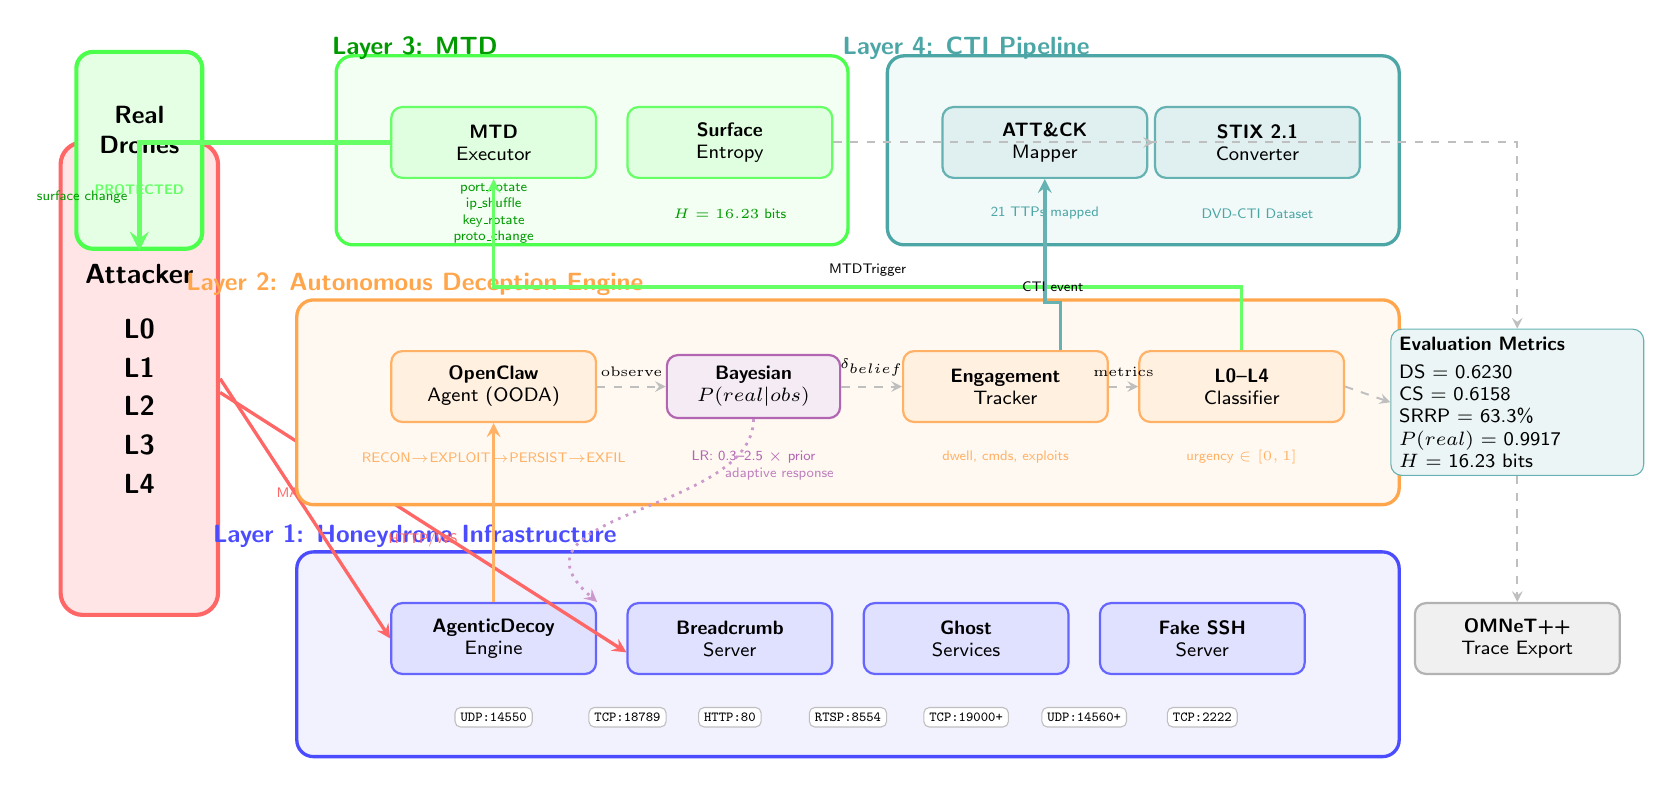
\begin{tikzpicture}[
    >=stealth,
    layer/.style={
        rectangle, rounded corners=6pt, draw=#1!70, fill=#1!5,
        line width=1.2pt, minimum height=2.8cm, align=center
    },
    comp/.style={
        rectangle, rounded corners=4pt, draw=#1!60, fill=#1!12,
        line width=0.8pt, minimum width=2.6cm, minimum height=0.9cm,
        align=center, font=\sffamily\scriptsize
    },
    port/.style={
        rectangle, rounded corners=2pt, draw=gray!50, fill=white,
        font=\ttfamily\tiny, inner sep=2pt
    },
    flow/.style={->, line width=1.2pt, draw=#1!60},
    dataflow/.style={->, line width=0.7pt, draw=gray!50, dashed},
    beliefbox/.style={
        rectangle, rounded corners=4pt, draw=violet!60, fill=violet!8,
        line width=0.8pt, font=\sffamily\scriptsize, align=center,
        minimum width=2.2cm, minimum height=0.8cm
    },
    metricbox/.style={
        rectangle, rounded corners=4pt, draw=teal!60, fill=teal!8,
        font=\sffamily\scriptsize, align=left, text width=3.0cm,
        inner sep=3pt
    },
]

% ═══════════════════════════════════════════════════════════════
% ATTACKER (left side)
% ═══════════════════════════════════════════════════════════════
\node[rectangle, rounded corners=8pt, draw=red!60, fill=red!10,
      line width=1.5pt, minimum width=2.0cm, minimum height=6cm,
      align=center, font=\sffamily\bfseries]
    (ATK) at (-2, 4.5) {Attacker\\[8pt]\romark{L0}\\[2pt]\romark{L1}\\[2pt]\romark{L2}\\[2pt]\romark{L3}\\[2pt]\romark{L4}};

% ═══════════════════════════════════════════════════════════════
% LAYER 1: Honeydrone Infrastructure (bottom)
% ═══════════════════════════════════════════════════════════════
\node[layer=blue, minimum width=14cm, minimum height=2.6cm] (L1) at (7, 1) {};
\node[font=\sffamily\bfseries\small, text=blue!70] at (1.5, 2.5) {Layer 1: Honeydrone Infrastructure};

% Components
\node[comp=blue] (engine) at (2.5, 1.2) {\textbf{AgenticDecoy}\\Engine};
\node[comp=blue] (bread)  at (5.5, 1.2) {\textbf{Breadcrumb}\\Server};
\node[comp=blue] (ghost)  at (8.5, 1.2) {\textbf{Ghost}\\Services};
\node[comp=blue] (ssh)    at (11.5, 1.2) {\textbf{Fake SSH}\\Server};

% Ports
\node[port] at (2.5, 0.2) {UDP:14550};
\node[port] at (4.2, 0.2) {TCP:18789};
\node[port] at (5.5, 0.2) {HTTP:80};
\node[port] at (7.0, 0.2) {RTSP:8554};
\node[port] at (8.5, 0.2) {TCP:19000+};
\node[port] at (10.0, 0.2) {UDP:14560+};
\node[port] at (11.5, 0.2) {TCP:2222};

% Attack arrows into Layer 1
\draw[flow=red] (ATK.east) -- node[above, font=\sffamily\tiny, text=red!60] {MAVLink} (engine.west);
\draw[flow=red] ([yshift=-5pt]ATK.east) -- node[below, font=\sffamily\tiny, text=red!60] {HTTP/WS} ([yshift=-5pt]bread.west);

% ═══════════════════════════════════════════════════════════════
% LAYER 2: Autonomous Deception (middle)
% ═══════════════════════════════════════════════════════════════
\node[layer=orange, minimum width=14cm, minimum height=2.6cm] (L2) at (7, 4.2) {};
\node[font=\sffamily\bfseries\small, text=orange!70] at (1.5, 5.7) {Layer 2: Autonomous Deception Engine};

\node[comp=orange] (ooda) at (2.5, 4.4) {\textbf{OpenClaw}\\Agent (OODA)};
\node[beliefbox]   (belief) at (5.8, 4.4) {\textbf{Bayesian}\\$P(\text{real}|\text{obs})$};
\node[comp=orange] (track) at (9.0, 4.4) {\textbf{Engagement}\\Tracker};
\node[comp=orange] (class) at (12.0, 4.4) {\textbf{L0--L4}\\Classifier};

% Subdetails
\node[font=\sffamily\tiny, text=orange!60] at (2.5, 3.5) {RECON$\to$EXPLOIT$\to$PERSIST$\to$EXFIL};
\node[font=\sffamily\tiny, text=violet!60] at (5.8, 3.5) {LR: 0.3--2.5 $\times$ prior};
\node[font=\sffamily\tiny, text=orange!60] at (9.0, 3.5) {dwell, cmds, exploits};
\node[font=\sffamily\tiny, text=orange!60] at (12.0, 3.5) {urgency $\in [0,1]$};

% Internal flows
\draw[flow=orange] (engine.north) -- (ooda.south);
\draw[dataflow] (ooda) -- node[above, font=\tiny] {observe} (belief);
\draw[dataflow] (belief) -- node[above, font=\tiny] {$\delta_{\text{belief}}$} (track);
\draw[dataflow] (track) -- node[above, font=\tiny] {metrics} (class);

% ═══════════════════════════════════════════════════════════════
% LAYER 3: MTD (top-left)
% ═══════════════════════════════════════════════════════════════
\node[layer=green, minimum width=6.5cm, minimum height=2.4cm] (L3) at (3.75, 7.4) {};
\node[font=\sffamily\bfseries\small, text=green!60!black] at (1.5, 8.7) {Layer 3: MTD};

\node[comp=green] (executor) at (2.5, 7.5) {\textbf{MTD}\\Executor};
\node[comp=green] (entropy) at (5.5, 7.5) {\textbf{Surface}\\Entropy};

\node[font=\sffamily\tiny, text=green!60!black, align=center] at (2.5, 6.6) {port\_rotate\\ip\_shuffle\\key\_rotate\\proto\_change};
\node[font=\sffamily\tiny, text=green!60!black] at (5.5, 6.6) {$H=16.23$ bits};

% MTD trigger from classifier
\draw[flow=green] (class.north) -- ++(0, 0.8) -| node[near start, above, font=\sffamily\tiny] {MTDTrigger} (executor.south);

% ═══════════════════════════════════════════════════════════════
% LAYER 4: CTI Pipeline (top-right)
% ═══════════════════════════════════════════════════════════════
\node[layer=teal, minimum width=6.5cm, minimum height=2.4cm] (L4) at (10.75, 7.4) {};
\node[font=\sffamily\bfseries\small, text=teal!70] at (8.5, 8.7) {Layer 4: CTI Pipeline};

\node[comp=teal] (parser) at (9.5, 7.5) {\textbf{ATT\&CK}\\Mapper};
\node[comp=teal] (stix)   at (12.2, 7.5) {\textbf{STIX 2.1}\\Converter};

\node[font=\sffamily\tiny, text=teal!70] at (9.5, 6.6) {21 TTPs mapped};
\node[font=\sffamily\tiny, text=teal!70] at (12.2, 6.6) {DVD-CTI Dataset};

% CTI flow
\draw[flow=teal] ([xshift=20pt]track.north) -- ++(0, 0.6) -| node[near start, above, font=\sffamily\tiny] {CTI event} (parser.south);
\draw[dataflow] (parser) -- (stix);

% ═══════════════════════════════════════════════════════════════
% METRICS OUTPUT (right side)
% ═══════════════════════════════════════════════════════════════
\node[metricbox] (metrics) at (15.5, 4.2) {
    \textbf{Evaluation Metrics}\\[2pt]
    DS = 0.6230\\
    CS = 0.6158\\
    SRRP = 63.3\%\\
    $P(\text{real})$ = 0.9917\\
    $H$ = 16.23 bits
};
\draw[dataflow] (class.east) -- (metrics.west);
\draw[dataflow] (entropy.east) -| (metrics.north);

% ═══════════════════════════════════════════════════════════════
% OMNeT++ Output (bottom-right)
% ═══════════════════════════════════════════════════════════════
\node[comp=gray] (omnet) at (15.5, 1.2) {\textbf{OMNeT++}\\Trace Export};
\draw[dataflow] (metrics.south) -- (omnet.north);

% ═══════════════════════════════════════════════════════════════
% REAL DRONES (protected, far left)
% ═══════════════════════════════════════════════════════════════
\node[rectangle, rounded corners=6pt, draw=green!70, fill=green!10,
      line width=1.5pt, minimum width=1.6cm, minimum height=2.5cm,
      align=center, font=\sffamily\bfseries\small]
    (REAL) at (-2, 7.4) {Real\\Drones\\[4pt]{\tiny\textcolor{green!60}{PROTECTED}}};

\draw[flow=green, line width=2pt] (executor.west) -| node[near end, left, font=\sffamily\tiny, text=green!60!black] {surface change} (REAL.south);

% ═══════════════════════════════════════════════════════════════
% Deception feedback loop (big curved arrow)
% ═════════════════════════════════════════════════════════���═════
\draw[->, line width=1pt, draw=violet!40, dotted]
    (belief.south) .. controls (5.8, 2.8) and (2.5, 2.8) .. (engine.north east)
    node[near start, right, font=\sffamily\tiny, text=violet!50] {adaptive response};

\end{tikzpicture}
}
\caption{MIRAGE-UAS 4-Layer 방어 아키텍처. 공격자 트래픽은 Layer~1의 허니드론 인프라에 유입되고, Layer~2의 자율 기만 엔진이 OODA 루프와 베이지안 믿음 추적으로 적응형 응답을 생성한다. Layer~3의 MTD는 공격자 레벨 기반 urgency에 따라 공격 표면을 재구성하며, Layer~4의 CTI 파이프라인은 공격 이벤트를 STIX 2.1 데이터셋으로 변환한다.}
\label{fig:defense}
\end{figure*}

% ═══════════════════════════════════════════════════════════════
\begin{figure*}[t]
\centering
\resizebox{\textwidth}{!}{%
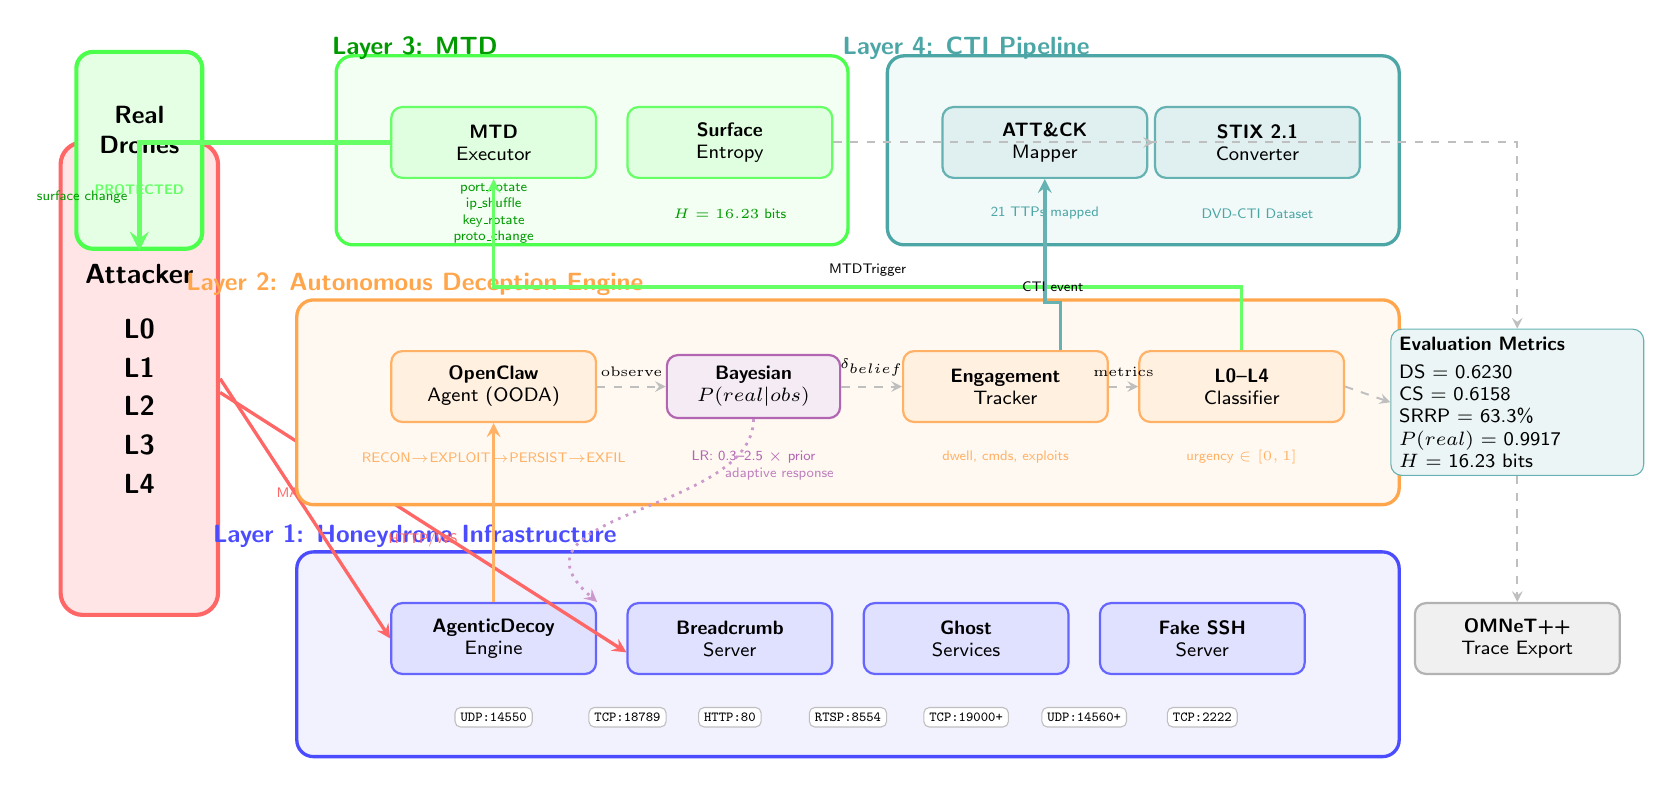
\begin{tikzpicture}[
    >=stealth,
    layer/.style={
        rectangle, rounded corners=6pt, draw=#1!70, fill=#1!5,
        line width=1.2pt, minimum height=2.8cm, align=center
    },
    comp/.style={
        rectangle, rounded corners=4pt, draw=#1!60, fill=#1!12,
        line width=0.8pt, minimum width=2.6cm, minimum height=0.9cm,
        align=center, font=\sffamily\scriptsize
    },
    port/.style={
        rectangle, rounded corners=2pt, draw=gray!50, fill=white,
        font=\ttfamily\tiny, inner sep=2pt
    },
    flow/.style={->, line width=1.2pt, draw=#1!60},
    dataflow/.style={->, line width=0.7pt, draw=gray!50, dashed},
    beliefbox/.style={
        rectangle, rounded corners=4pt, draw=violet!60, fill=violet!8,
        line width=0.8pt, font=\sffamily\scriptsize, align=center,
        minimum width=2.2cm, minimum height=0.8cm
    },
    metricbox/.style={
        rectangle, rounded corners=4pt, draw=teal!60, fill=teal!8,
        font=\sffamily\scriptsize, align=left, text width=3.0cm,
        inner sep=3pt
    },
]

% ═══════════════════════════════════════════════════════════════
% ATTACKER (left side)
% ═══════════════════════════════════════════════════════════════
\node[rectangle, rounded corners=8pt, draw=red!60, fill=red!10,
      line width=1.5pt, minimum width=2.0cm, minimum height=6cm,
      align=center, font=\sffamily\bfseries]
    (ATK) at (-2, 4.5) {Attacker\\[8pt]\romark{L0}\\[2pt]\romark{L1}\\[2pt]\romark{L2}\\[2pt]\romark{L3}\\[2pt]\romark{L4}};

% ═══════════════════════════════════════════════════════════════
% LAYER 1: Honeydrone Infrastructure (bottom)
% ═══════════════════════════════════════════════════════════════
\node[layer=blue, minimum width=14cm, minimum height=2.6cm] (L1) at (7, 1) {};
\node[font=\sffamily\bfseries\small, text=blue!70] at (1.5, 2.5) {Layer 1: Honeydrone Infrastructure};

% Components
\node[comp=blue] (engine) at (2.5, 1.2) {\textbf{AgenticDecoy}\\Engine};
\node[comp=blue] (bread)  at (5.5, 1.2) {\textbf{Breadcrumb}\\Server};
\node[comp=blue] (ghost)  at (8.5, 1.2) {\textbf{Ghost}\\Services};
\node[comp=blue] (ssh)    at (11.5, 1.2) {\textbf{Fake SSH}\\Server};

% Ports
\node[port] at (2.5, 0.2) {UDP:14550};
\node[port] at (4.2, 0.2) {TCP:18789};
\node[port] at (5.5, 0.2) {HTTP:80};
\node[port] at (7.0, 0.2) {RTSP:8554};
\node[port] at (8.5, 0.2) {TCP:19000+};
\node[port] at (10.0, 0.2) {UDP:14560+};
\node[port] at (11.5, 0.2) {TCP:2222};

% Attack arrows into Layer 1
\draw[flow=red] (ATK.east) -- node[above, font=\sffamily\tiny, text=red!60] {MAVLink} (engine.west);
\draw[flow=red] ([yshift=-5pt]ATK.east) -- node[below, font=\sffamily\tiny, text=red!60] {HTTP/WS} ([yshift=-5pt]bread.west);

% ═══════════════════════════════════════════════════════════════
% LAYER 2: Autonomous Deception (middle)
% ═══════════════════════════════════════════════════════════════
\node[layer=orange, minimum width=14cm, minimum height=2.6cm] (L2) at (7, 4.2) {};
\node[font=\sffamily\bfseries\small, text=orange!70] at (1.5, 5.7) {Layer 2: Autonomous Deception Engine};

\node[comp=orange] (ooda) at (2.5, 4.4) {\textbf{OpenClaw}\\Agent (OODA)};
\node[beliefbox]   (belief) at (5.8, 4.4) {\textbf{Bayesian}\\$P(\text{real}|\text{obs})$};
\node[comp=orange] (track) at (9.0, 4.4) {\textbf{Engagement}\\Tracker};
\node[comp=orange] (class) at (12.0, 4.4) {\textbf{L0--L4}\\Classifier};

% Subdetails
\node[font=\sffamily\tiny, text=orange!60] at (2.5, 3.5) {RECON$\to$EXPLOIT$\to$PERSIST$\to$EXFIL};
\node[font=\sffamily\tiny, text=violet!60] at (5.8, 3.5) {LR: 0.3--2.5 $\times$ prior};
\node[font=\sffamily\tiny, text=orange!60] at (9.0, 3.5) {dwell, cmds, exploits};
\node[font=\sffamily\tiny, text=orange!60] at (12.0, 3.5) {urgency $\in [0,1]$};

% Internal flows
\draw[flow=orange] (engine.north) -- (ooda.south);
\draw[dataflow] (ooda) -- node[above, font=\tiny] {observe} (belief);
\draw[dataflow] (belief) -- node[above, font=\tiny] {$\delta_{\text{belief}}$} (track);
\draw[dataflow] (track) -- node[above, font=\tiny] {metrics} (class);

% ═══════════════════════════════════════════════════════════════
% LAYER 3: MTD (top-left)
% ═══════════════════════════════════════════════════════════════
\node[layer=green, minimum width=6.5cm, minimum height=2.4cm] (L3) at (3.75, 7.4) {};
\node[font=\sffamily\bfseries\small, text=green!60!black] at (1.5, 8.7) {Layer 3: MTD};

\node[comp=green] (executor) at (2.5, 7.5) {\textbf{MTD}\\Executor};
\node[comp=green] (entropy) at (5.5, 7.5) {\textbf{Surface}\\Entropy};

\node[font=\sffamily\tiny, text=green!60!black, align=center] at (2.5, 6.6) {port\_rotate\\ip\_shuffle\\key\_rotate\\proto\_change};
\node[font=\sffamily\tiny, text=green!60!black] at (5.5, 6.6) {$H=16.23$ bits};

% MTD trigger from classifier
\draw[flow=green] (class.north) -- ++(0, 0.8) -| node[near start, above, font=\sffamily\tiny] {MTDTrigger} (executor.south);

% ═══════════════════════════════════════════════════════════════
% LAYER 4: CTI Pipeline (top-right)
% ═══════════════════════════════════════════════════════════════
\node[layer=teal, minimum width=6.5cm, minimum height=2.4cm] (L4) at (10.75, 7.4) {};
\node[font=\sffamily\bfseries\small, text=teal!70] at (8.5, 8.7) {Layer 4: CTI Pipeline};

\node[comp=teal] (parser) at (9.5, 7.5) {\textbf{ATT\&CK}\\Mapper};
\node[comp=teal] (stix)   at (12.2, 7.5) {\textbf{STIX 2.1}\\Converter};

\node[font=\sffamily\tiny, text=teal!70] at (9.5, 6.6) {21 TTPs mapped};
\node[font=\sffamily\tiny, text=teal!70] at (12.2, 6.6) {DVD-CTI Dataset};

% CTI flow
\draw[flow=teal] ([xshift=20pt]track.north) -- ++(0, 0.6) -| node[near start, above, font=\sffamily\tiny] {CTI event} (parser.south);
\draw[dataflow] (parser) -- (stix);

% ═══════════════════════════════════════════════════════════════
% METRICS OUTPUT (right side)
% ═══════════════════════════════════════════════════════════════
\node[metricbox] (metrics) at (15.5, 4.2) {
    \textbf{Evaluation Metrics}\\[2pt]
    DS = 0.6230\\
    CS = 0.6158\\
    SRRP = 63.3\%\\
    $P(\text{real})$ = 0.9917\\
    $H$ = 16.23 bits
};
\draw[dataflow] (class.east) -- (metrics.west);
\draw[dataflow] (entropy.east) -| (metrics.north);

% ═══════════════════════════════════════════════════════════════
% OMNeT++ Output (bottom-right)
% ═══════════════════════════════════════════════════════════════
\node[comp=gray] (omnet) at (15.5, 1.2) {\textbf{OMNeT++}\\Trace Export};
\draw[dataflow] (metrics.south) -- (omnet.north);

% ═══════════════════════════════════════════════════════════════
% REAL DRONES (protected, far left)
% ═══════════════════════════════════════════════════════════════
\node[rectangle, rounded corners=6pt, draw=green!70, fill=green!10,
      line width=1.5pt, minimum width=1.6cm, minimum height=2.5cm,
      align=center, font=\sffamily\bfseries\small]
    (REAL) at (-2, 7.4) {Real\\Drones\\[4pt]{\tiny\textcolor{green!60}{PROTECTED}}};

\draw[flow=green, line width=2pt] (executor.west) -| node[near end, left, font=\sffamily\tiny, text=green!60!black] {surface change} (REAL.south);

% ═══════════════════════════════════════════════════════════════
% Deception feedback loop (big curved arrow)
% ═════════════════════════════════════════════════════════���═════
\draw[->, line width=1pt, draw=violet!40, dotted]
    (belief.south) .. controls (5.8, 2.8) and (2.5, 2.8) .. (engine.north east)
    node[near start, right, font=\sffamily\tiny, text=violet!50] {adaptive response};

\end{tikzpicture}
}
\caption{MIRAGE-UAS 4-Layer 방어 아키텍처. 공격자 트래픽은 Layer~1의 허니드론 인프라에 유입되고, Layer~2의 자율 기만 엔진이 OODA 루프와 베이지안 믿음 추적으로 적응형 응답을 생성한다. Layer~3의 MTD는 공격자 레벨 기반 urgency에 따라 공격 표면을 재구성하며, Layer~4의 CTI 파이프라인은 공격 이벤트를 STIX 2.1 데이터셋으로 변환한다.}
\label{fig:defense}
\end{figure*}

% ═══════════════════════════════════════════════════════════════
\begin{figure*}[t]
\centering
\resizebox{\textwidth}{!}{%
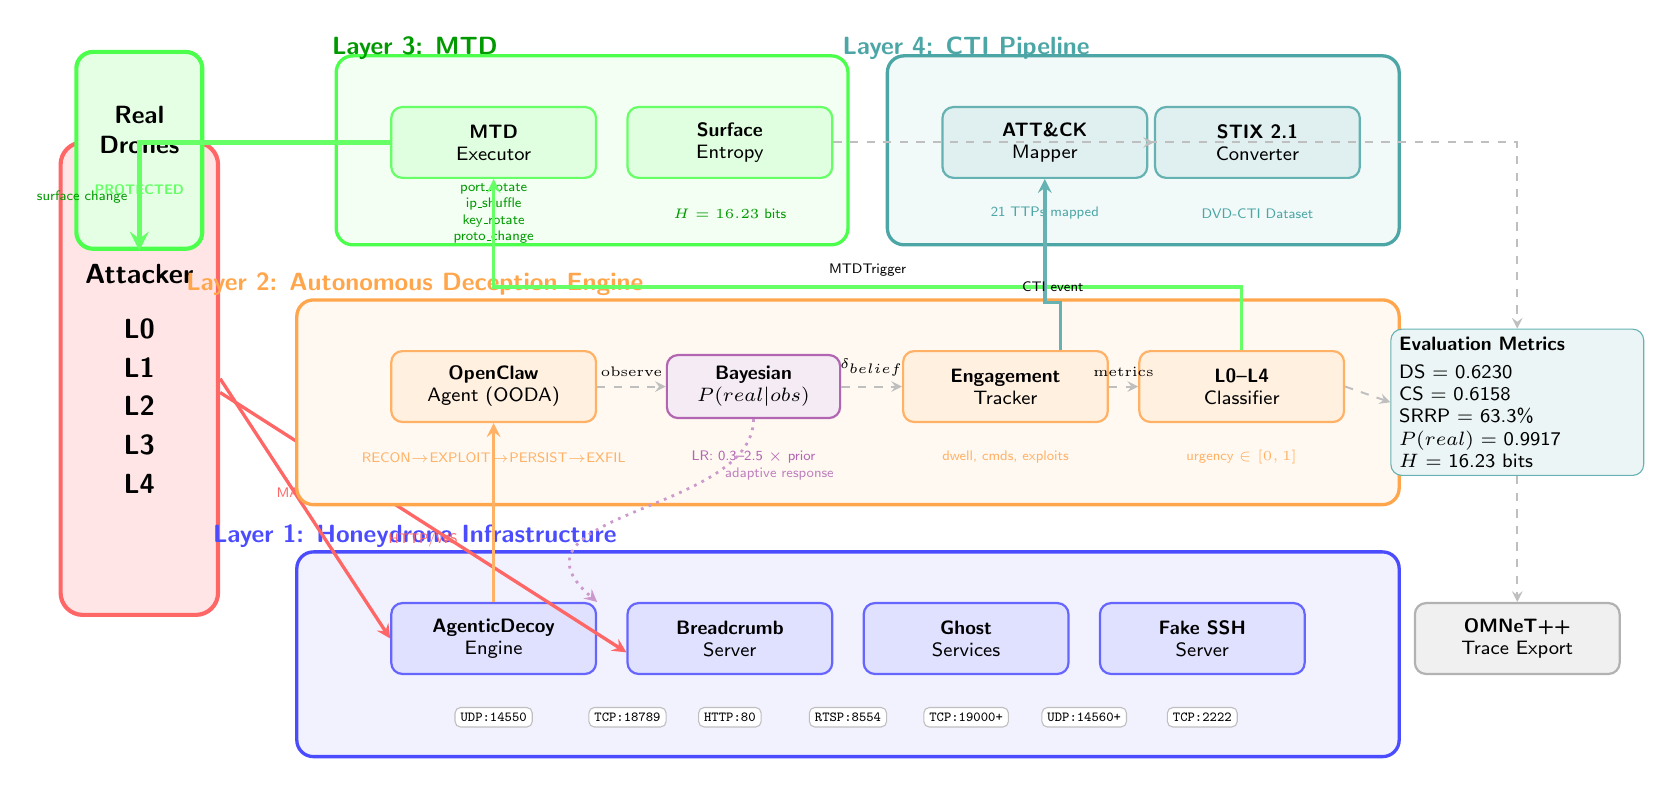
\begin{tikzpicture}[
    >=stealth,
    layer/.style={
        rectangle, rounded corners=6pt, draw=#1!70, fill=#1!5,
        line width=1.2pt, minimum height=2.8cm, align=center
    },
    comp/.style={
        rectangle, rounded corners=4pt, draw=#1!60, fill=#1!12,
        line width=0.8pt, minimum width=2.6cm, minimum height=0.9cm,
        align=center, font=\sffamily\scriptsize
    },
    port/.style={
        rectangle, rounded corners=2pt, draw=gray!50, fill=white,
        font=\ttfamily\tiny, inner sep=2pt
    },
    flow/.style={->, line width=1.2pt, draw=#1!60},
    dataflow/.style={->, line width=0.7pt, draw=gray!50, dashed},
    beliefbox/.style={
        rectangle, rounded corners=4pt, draw=violet!60, fill=violet!8,
        line width=0.8pt, font=\sffamily\scriptsize, align=center,
        minimum width=2.2cm, minimum height=0.8cm
    },
    metricbox/.style={
        rectangle, rounded corners=4pt, draw=teal!60, fill=teal!8,
        font=\sffamily\scriptsize, align=left, text width=3.0cm,
        inner sep=3pt
    },
]

% ═══════════════════════════════════════════════════════════════
% ATTACKER (left side)
% ═══════════════════════════════════════════════════════════════
\node[rectangle, rounded corners=8pt, draw=red!60, fill=red!10,
      line width=1.5pt, minimum width=2.0cm, minimum height=6cm,
      align=center, font=\sffamily\bfseries]
    (ATK) at (-2, 4.5) {Attacker\\[8pt]\romark{L0}\\[2pt]\romark{L1}\\[2pt]\romark{L2}\\[2pt]\romark{L3}\\[2pt]\romark{L4}};

% ═══════════════════════════════════════════════════════════════
% LAYER 1: Honeydrone Infrastructure (bottom)
% ═══════════════════════════════════════════════════════════════
\node[layer=blue, minimum width=14cm, minimum height=2.6cm] (L1) at (7, 1) {};
\node[font=\sffamily\bfseries\small, text=blue!70] at (1.5, 2.5) {Layer 1: Honeydrone Infrastructure};

% Components
\node[comp=blue] (engine) at (2.5, 1.2) {\textbf{AgenticDecoy}\\Engine};
\node[comp=blue] (bread)  at (5.5, 1.2) {\textbf{Breadcrumb}\\Server};
\node[comp=blue] (ghost)  at (8.5, 1.2) {\textbf{Ghost}\\Services};
\node[comp=blue] (ssh)    at (11.5, 1.2) {\textbf{Fake SSH}\\Server};

% Ports
\node[port] at (2.5, 0.2) {UDP:14550};
\node[port] at (4.2, 0.2) {TCP:18789};
\node[port] at (5.5, 0.2) {HTTP:80};
\node[port] at (7.0, 0.2) {RTSP:8554};
\node[port] at (8.5, 0.2) {TCP:19000+};
\node[port] at (10.0, 0.2) {UDP:14560+};
\node[port] at (11.5, 0.2) {TCP:2222};

% Attack arrows into Layer 1
\draw[flow=red] (ATK.east) -- node[above, font=\sffamily\tiny, text=red!60] {MAVLink} (engine.west);
\draw[flow=red] ([yshift=-5pt]ATK.east) -- node[below, font=\sffamily\tiny, text=red!60] {HTTP/WS} ([yshift=-5pt]bread.west);

% ═══════════════════════════════════════════════════════════════
% LAYER 2: Autonomous Deception (middle)
% ═══════════════════════════════════════════════════════════════
\node[layer=orange, minimum width=14cm, minimum height=2.6cm] (L2) at (7, 4.2) {};
\node[font=\sffamily\bfseries\small, text=orange!70] at (1.5, 5.7) {Layer 2: Autonomous Deception Engine};

\node[comp=orange] (ooda) at (2.5, 4.4) {\textbf{OpenClaw}\\Agent (OODA)};
\node[beliefbox]   (belief) at (5.8, 4.4) {\textbf{Bayesian}\\$P(\text{real}|\text{obs})$};
\node[comp=orange] (track) at (9.0, 4.4) {\textbf{Engagement}\\Tracker};
\node[comp=orange] (class) at (12.0, 4.4) {\textbf{L0--L4}\\Classifier};

% Subdetails
\node[font=\sffamily\tiny, text=orange!60] at (2.5, 3.5) {RECON$\to$EXPLOIT$\to$PERSIST$\to$EXFIL};
\node[font=\sffamily\tiny, text=violet!60] at (5.8, 3.5) {LR: 0.3--2.5 $\times$ prior};
\node[font=\sffamily\tiny, text=orange!60] at (9.0, 3.5) {dwell, cmds, exploits};
\node[font=\sffamily\tiny, text=orange!60] at (12.0, 3.5) {urgency $\in [0,1]$};

% Internal flows
\draw[flow=orange] (engine.north) -- (ooda.south);
\draw[dataflow] (ooda) -- node[above, font=\tiny] {observe} (belief);
\draw[dataflow] (belief) -- node[above, font=\tiny] {$\delta_{\text{belief}}$} (track);
\draw[dataflow] (track) -- node[above, font=\tiny] {metrics} (class);

% ═══════════════════════════════════════════════════════════════
% LAYER 3: MTD (top-left)
% ═══════════════════════════════════════════════════════════════
\node[layer=green, minimum width=6.5cm, minimum height=2.4cm] (L3) at (3.75, 7.4) {};
\node[font=\sffamily\bfseries\small, text=green!60!black] at (1.5, 8.7) {Layer 3: MTD};

\node[comp=green] (executor) at (2.5, 7.5) {\textbf{MTD}\\Executor};
\node[comp=green] (entropy) at (5.5, 7.5) {\textbf{Surface}\\Entropy};

\node[font=\sffamily\tiny, text=green!60!black, align=center] at (2.5, 6.6) {port\_rotate\\ip\_shuffle\\key\_rotate\\proto\_change};
\node[font=\sffamily\tiny, text=green!60!black] at (5.5, 6.6) {$H=16.23$ bits};

% MTD trigger from classifier
\draw[flow=green] (class.north) -- ++(0, 0.8) -| node[near start, above, font=\sffamily\tiny] {MTDTrigger} (executor.south);

% ═══════════════════════════════════════════════════════════════
% LAYER 4: CTI Pipeline (top-right)
% ═══════════════════════════════════════════════════════════════
\node[layer=teal, minimum width=6.5cm, minimum height=2.4cm] (L4) at (10.75, 7.4) {};
\node[font=\sffamily\bfseries\small, text=teal!70] at (8.5, 8.7) {Layer 4: CTI Pipeline};

\node[comp=teal] (parser) at (9.5, 7.5) {\textbf{ATT\&CK}\\Mapper};
\node[comp=teal] (stix)   at (12.2, 7.5) {\textbf{STIX 2.1}\\Converter};

\node[font=\sffamily\tiny, text=teal!70] at (9.5, 6.6) {21 TTPs mapped};
\node[font=\sffamily\tiny, text=teal!70] at (12.2, 6.6) {DVD-CTI Dataset};

% CTI flow
\draw[flow=teal] ([xshift=20pt]track.north) -- ++(0, 0.6) -| node[near start, above, font=\sffamily\tiny] {CTI event} (parser.south);
\draw[dataflow] (parser) -- (stix);

% ═══════════════════════════════════════════════════════════════
% METRICS OUTPUT (right side)
% ═══════════════════════════════════════════════════════════════
\node[metricbox] (metrics) at (15.5, 4.2) {
    \textbf{Evaluation Metrics}\\[2pt]
    DS = 0.6230\\
    CS = 0.6158\\
    SRRP = 63.3\%\\
    $P(\text{real})$ = 0.9917\\
    $H$ = 16.23 bits
};
\draw[dataflow] (class.east) -- (metrics.west);
\draw[dataflow] (entropy.east) -| (metrics.north);

% ═══════════════════════════════════════════════════════════════
% OMNeT++ Output (bottom-right)
% ═══════════════════════════════════════════════════════════════
\node[comp=gray] (omnet) at (15.5, 1.2) {\textbf{OMNeT++}\\Trace Export};
\draw[dataflow] (metrics.south) -- (omnet.north);

% ═══════════════════════════════════════════════════════════════
% REAL DRONES (protected, far left)
% ═══════════════════════════════════════════════════════════════
\node[rectangle, rounded corners=6pt, draw=green!70, fill=green!10,
      line width=1.5pt, minimum width=1.6cm, minimum height=2.5cm,
      align=center, font=\sffamily\bfseries\small]
    (REAL) at (-2, 7.4) {Real\\Drones\\[4pt]{\tiny\textcolor{green!60}{PROTECTED}}};

\draw[flow=green, line width=2pt] (executor.west) -| node[near end, left, font=\sffamily\tiny, text=green!60!black] {surface change} (REAL.south);

% ═══════════════════════════════════════════════════════════════
% Deception feedback loop (big curved arrow)
% ═════════════════════════════════════════════════════════���═════
\draw[->, line width=1pt, draw=violet!40, dotted]
    (belief.south) .. controls (5.8, 2.8) and (2.5, 2.8) .. (engine.north east)
    node[near start, right, font=\sffamily\tiny, text=violet!50] {adaptive response};

\end{tikzpicture}
}
\caption{MIRAGE-UAS 4-Layer 방어 아키텍처. 공격자 트래픽은 Layer~1의 허니드론 인프라에 유입되고, Layer~2의 자율 기만 엔진이 OODA 루프와 베이지안 믿음 추적으로 적응형 응답을 생성한다. Layer~3의 MTD는 공격자 레벨 기반 urgency에 따라 공격 표면을 재구성하며, Layer~4의 CTI 파이프라인은 공격 이벤트를 STIX 2.1 데이터셋으로 변환한다.}
\label{fig:defense}
\end{figure*}
   % Figure: Defense Architecture
%
% Notes:
%   - fig_ooda_loop:    \begin{figure}[t]   (single column)
%   - fig_attack_model: \begin{figure}[t]   (single column)
%   - fig_defense_arch: \begin{figure*}[t]  (double column, full width)
% ═══════════════════════════════════════════════════════════════
